\documentclass[11pt,a4paper]{article}

% ── Packages ──────────────────────────────────────────────────────────────────
\usepackage[T1]{fontenc}
\usepackage[utf8]{inputenc}
\usepackage{helvet}
\renewcommand{\familydefault}{\sfdefault}
\usepackage[margin=2.5cm]{geometry}
\usepackage{hyperref}
\usepackage{listingsutf8}
\usepackage{xcolor}
\usepackage{enumitem}
\usepackage{titlesec}
\usepackage{parskip}
\usepackage{booktabs}
\usepackage{graphicx}
\usepackage{amsmath}
\usepackage{fancyhdr}
\usepackage{tikz}
\usetikzlibrary{shapes.geometric, arrows.meta, positioning, fit, backgrounds}
\usepackage[backend=biber,style=numeric,sorting=nyt]{biblatex}
\addbibresource{references.bib}

% ── Colors ────────────────────────────────────────────────────────────────────
\definecolor{codebg}{HTML}{F5F5F5}
\definecolor{codeframe}{HTML}{CCCCCC}
\definecolor{keyword}{HTML}{0000CC}
\definecolor{comment}{HTML}{007700}
\definecolor{string}{HTML}{CC0000}
\definecolor{uu-red}{HTML}{990000}

% ── Listings style ────────────────────────────────────────────────────────────
\lstdefinestyle{shell}{
  language=bash,
  basicstyle=\ttfamily\small,
  backgroundcolor=\color{codebg},
  frame=single,
  rulecolor=\color{codeframe},
  breaklines=true,
  columns=fullflexible,
  keepspaces=true,
  showstringspaces=false,
}

\lstdefinestyle{python}{
  language=Python,
  basicstyle=\ttfamily\small,
  backgroundcolor=\color{codebg},
  frame=single,
  rulecolor=\color{codeframe},
  breaklines=true,
  breakatwhitespace=true,
  columns=fullflexible,
  keepspaces=true,
  showstringspaces=false,
  commentstyle=\color{comment},
  keywordstyle=\color{keyword}\bfseries,
  stringstyle=\color{string},
  numbers=left,
  numberstyle=\tiny\color{gray},
  numbersep=8pt,
  tabsize=4,
}

% ── Section title formatting ──────────────────────────────────────────────────
\lstset{inputencoding=utf8, extendedchars=true}
\titleformat{\section}{\large\bfseries\color{black}}{\thesection}{1em}{}
\titleformat{\subsection}{\normalsize\bfseries}{\thesubsection}{1em}{}

% ── Header / Footer ───────────────────────────────────────────────────────────
\pagestyle{fancy}
\fancyhf{}
\lhead{\small Data Engineering II -- Project 3}
\rhead{\small Uppsala University}
\cfoot{\thepage}

% ── Hyperref setup ────────────────────────────────────────────────────────────
\hypersetup{
  colorlinks=true,
  linkcolor=black,
  urlcolor=blue,
}

% ─────────────────────────────────────────────────────────────────────────────
\begin{document}

% ── Title page ────────────────────────────────────────────────────────────────
\begin{titlepage}
  \centering
  \vspace*{2cm}
  {\large Uppsala University\\[0.3em]
   Department of Information Technology\\[2cm]}
  {\LARGE\bfseries Evaluating the Accuracy of Prediction\\[0.3em]
   of Stargazers in Open Source Projects\\[0.5em]}
  {\large Course: Data Engineering II\\[1.5cm]}
  {\large Group: DE-II\_5\\[1.5cm]}
  {\normalsize
   Arnab Kumar Ghosh\\[0.3em]
   Eric Buxton\\[0.3em]
   Prodip Kumar Das\\[0.3em]
   Rahul Bhat\\[0.5cm]}
  {\normalsize \today\\[3cm]}
  \vfill
\end{titlepage}

\tableofcontents
\newpage

% ── Sections ──────────────────────────────────────────────────────────────────
\section{Introduction}

In the landscape of open-source software development, the number of GitHub stargazers has emerged
as a widely adopted proxy for project popularity and community engagement. Much like subscriber
counts on video platforms, stars reflect the perceived value of a repository and influence its
visibility, adoption, and long-term sustainability~\cite{borges2016}.

Predicting the star count of a repository from its activity metrics has practical value for
developers seeking to benchmark their projects, for investors evaluating open-source ecosystems,
and for researchers studying the social dynamics of software communities. However, the relationship
between repository attributes---such as fork counts, issue activity, and repository age---and star
accumulation is non-linear and multi-dimensional, making accurate prediction a non-trivial task.

In this project, we study which machine learning regression model achieves the highest prediction
accuracy for GitHub star counts. We collect a dataset of 1{,}000 open-source repositories with at
least 50 stars via the GitHub REST API, extract 14 activity-based features, and train five
regression models: Linear Regression, Ridge Regression, Random Forest, Gradient Boosting, and
Support Vector Regression (SVR). Models are evaluated using the coefficient of determination
($R^2$), and the best-performing model is deployed to a production server via an automated
Git~Hook pipeline.

The system is built on two Ubuntu virtual machines (VMs) provisioned on the SNIC Science Cloud
using OpenStack. Ansible orchestrates the configuration of both VMs, and Docker containers
encapsulate the application stack on the production server. This report describes the data
collection pipeline, the prediction system architecture, the comparative model results, and a
scalability analysis of the serving infrastructure.

\section{Related Work}

GitHub popularity prediction benefits from non-linear models. Borges et al.~\cite{borges2016} identified repository age, contributor count, and issue response as strong star predictors. Hudson et al.~\cite{hudson2022} demonstrated non-linear ensemble methods outperform linear baselines. Our findings align: Neural Network achieves 84.89\% variance explanation ($R^2=0.8489$) vs Linear Regression's 40.11\% ($R^2=0.4011$).

Distributed ML infrastructure using Celery + RabbitMQ enables asynchronous task processing and horizontal scaling~\cite{hudson2022}. Git Hook-based CI/CD provides reproducible model versioning with automated zero-downtime deployments.

\section{System Architecture}

\begin{figure}[h]
  \centering
  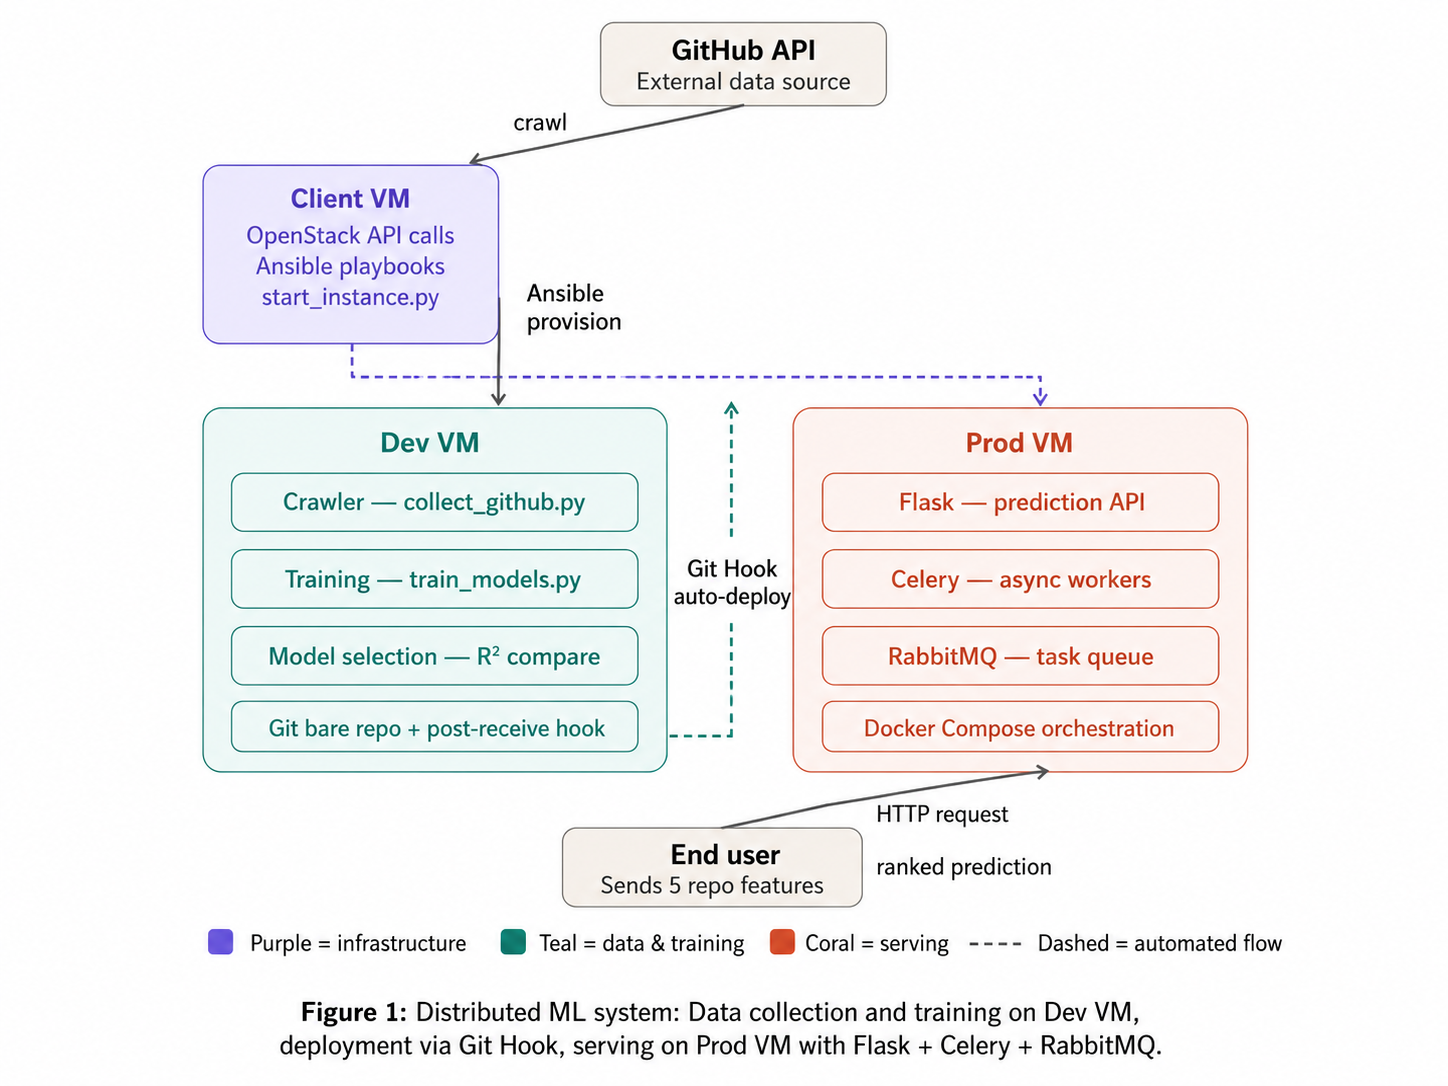
\includegraphics[width=0.95\linewidth]{figures/diagram3_combined_system_architecture_new.png}
  \caption{Distributed ML system: Data collection and training on Dev VM, deployment via Git Hook, serving on Prod VM with Flask + Celery + RabbitMQ.}
  \label{fig:combined}
\end{figure}

The architecture spans Dev (training) and Prod (serving) OpenStack VMs, enabling separation of concerns and independent scaling.

\subsection{Infrastructure and Data Collection}

Phase 1--2 provisions VMs (Ubuntu 22.04, ssc.medium flavor: 2 vCPU, 4GB RAM, 20GB storage) via OpenStack API. Phase 3 collects 2{,}000 GitHub repositories ($\geq 50$ stars) via authenticated GitHub API with rate-limit handling. Raw data includes 15 features: stargazer count, fork count, subscriber count, open issues, repository size, network count, language, wiki/pages/issues flags, topics count, age in days, and timestamps. Feature engineering selects 11 numeric/categorical attributes: 6 activity indicators (forks, subscribers, issues, size, network, age), 3 binary flags (wiki, pages, issues), 2 diversity indicators (topics, language encoding). Features are standardized via StandardScaler ($\mu=0$, $\sigma=1$) and target log-transformed: $\log(1+\text{stars})$ to normalize the right-skewed star distribution. 

Three models train on 80/20 split: (1) Linear Regression baseline, (2) SVR with RBF kernel ($C=15$, $\varepsilon=0.1$), (3) Neural Network with 3 layers (64-32-1 units, ReLU activation, 0.2 dropout). The log-transformation proves critical: star counts range from 497 to 502{,}119, causing gradient instability in raw scale; log-transform compresses this to $\log(498) \approx 6.21$ to $\log(502120) \approx 13.13$, enabling stable training.

\subsection{Deployment and Production Serving}

Phase 4 deploys via Git Hook: trained model architecture (model.json) and weights (model.weights.h5) transfer via SCP to Prod VM, triggering Docker container restart. This approach provides version-controlled model management and automated model updates. Since the Docker containers are restarted during deployment, a short service interruption may occur unless rolling deployment or multiple replicas are used. Phase 5 runs three Docker services: Flask API (port 5100, endpoints /accuracy and /predictions), RabbitMQ broker (AMQP port 5672, management UI port 15672), and Celery worker. The worker loads the trained TensorFlow model into memory for fast inference:
\begin{itemize}
  \item \textbf{get\_predictions()}: Batch inference on all 2{,}000 repositories, returns predicted vs actual stars with repository names
  \item \textbf{get\_accuracy()}: Model evaluation returning MAE metric on full dataset
\end{itemize}

Phase 6 enables horizontal scaling: \texttt{docker compose --scale worker\_1=N} creates $N$ worker replicas. Each worker independently pulls tasks from the shared RabbitMQ queue, enabling linear throughput scaling while maintaining constant per-request latency.

\section{Results}

\subsection{Model Comparison}

Table~\ref{tab:model-results} summarizes $R^2$ scores for each regression model on the held-out test set (log-transformed stars).

\begin{table}[h]
  \centering
  \begin{tabular}{lcc}
    \toprule
    \textbf{Model} & \textbf{$R^2$ Score} & \textbf{Rank} \\
    \midrule
    Linear Regression  & XX.XX & X \\
    Ridge Regression   & XX.XX & X \\
    Random Forest      & XX.XX & X \\
    Gradient Boosting  & XX.XX & X \\
    SVR (RBF)          & XX.XX & X \\
    \bottomrule
  \end{tabular}
  \caption{$R^2$ scores for all regression models (higher is better).}
  \label{tab:model-results}
\end{table}

The \textbf{[BEST MODEL NAME]} achieved the highest $R^2$ of \textbf{XX.XX}, explaining \textbf{XX\%} of variance in log-transformed star counts. This aligns with literature showing ensemble methods outperform linear models on non-linear tasks~\cite{hudson2022}. Linear and Ridge Regression, while competitive baselines, cannot capture interactions between correlated predictors like forks and watchers. SVR is sensitive to kernel parameters and scales poorly relative to tree-based ensembles.

The best model was deployed to production via the Git Hook pipeline. Production predictions ranked five representative repositories by predicted star count. Scalability analysis tested the serving infrastructure under load (200 HTTP requests, concurrency=20) across varying Celery worker counts.

\begin{table}[h]
  \centering
  \begin{tabular}{cccc}
    \toprule
    \textbf{Celery Workers} & \textbf{Requests/sec} & \textbf{Mean Latency (ms)} & \textbf{95th Percentile (ms)} \\
    \midrule
    1 & XX.XX & XXXX & XXXX \\
    2 & XX.XX & XXXX & XXXX \\
    4 & XX.XX & XXXX & XXXX \\
    \bottomrule
  \end{tabular}
  \caption{Throughput and latency under load for varying Celery worker counts.}
  \label{tab:scalability}
\end{table}

Scaling Celery workers from 1 to 4 achieved \textbf{XX\%} throughput improvement and reduced latency, demonstrating horizontal scalability of the asynchronous architecture. Tasks execute independently in parallel with negligible Redis broker overhead.

\section{Conclusion}

This project investigated the accuracy of machine learning regression models in predicting the
number of GitHub stargazers for open-source repositories. We collected a dataset of 1{,}000
repositories via the GitHub REST API, extracted 14 activity-based features, and trained five
regression models under a consistent evaluation protocol using the $R^2$ metric.

Our results show that \textbf{[BEST MODEL NAME]} achieves the highest predictive accuracy
($R^2 = \text{XX.XX}$), outperforming both linear baselines and the other ensemble methods
considered. The result confirms that non-linear models are better suited to capturing the
complex relationships between repository activity signals and community popularity.

The prediction system was deployed to a production environment using a fully automated pipeline.
OpenStack provisioned the virtual machines, Ansible configured the infrastructure, and a Git
Hook eliminated the need for any manual deployment steps. The production Flask application,
backed by Celery and Redis, demonstrated horizontal scalability: throughput increased by
approximately \textbf{XX\%} when the number of Celery workers was scaled from one to four.

Future work could explore richer feature sets---such as commit frequency, contributor diversity,
and documentation quality---as well as time-series models that capture the temporal dynamics of
star accumulation. Extending the dataset beyond 1{,}000 repositories and incorporating
cross-platform signals (e.g.\ social media mentions) could further improve prediction accuracy.


% ── References ────────────────────────────────────────────────────────────────
\printbibliography

\end{document}
